\documentclass[a4paper,10pt]{article}
%\documentclass[a4paper,10pt]{scrartcl}

\usepackage[utf8]{inputenc}
\usepackage{amsmath}
\usepackage{listings}
\usepackage{hyperref}
\usepackage{catoptions}
\usepackage[margin=1in]{geometry}
\usepackage{color}
\usepackage{soul}
\usepackage{float}
\usepackage{framed}
\usepackage[sc]{mathpazo}
\linespread{1.20}         % Palatino needs more leading (space between lines)
\usepackage[T1]{fontenc}
\usepackage{microtype}
\usepackage{enumerate}
\usepackage{courier}
\usepackage{graphicx}
\usepackage{xfrac}
\usepackage{enumitem}

\newcommand{\authorbd}{Bas Dado (4033736)}
\newcommand{\authoroh}{Olivier Hokke (1352679)}
\newcommand{\authortr}{Tom Runia (1517996)}
\newcommand{\authoras}{Arnold Schutter (4260724)}
\newcommand{\authortv}{Tom Viering (4333055)}
\newcommand{\maintitle}{Artificial Intelligence}
\newcommand{\subtitle}{BOAconstructor -- An Automated Negotiation Agent}

\title{\maintitle\\\subtitle}
\author{\authorbd\\\authoroh\\\authortr\\\authoras\\\authortv}
\date{\today}

\pdfinfo{%
  /Title    (\maintitle - \subtitle)
  /Author   (\authorbd, \authoroh, \authortr, \authoras, \authortv)
  /Creator  (\authorbd, \authoroh, \authortr, \authoras, \authortv)
  /Producer (\authorbd, \authoroh, \authortr, \authoras, \authortv)
  /Subject  (Automated Negotiation)
  /Keywords (Automated Negotiation, Genius, Bidding Strategy, Acceptance Strategy, Opponent Model, Opponent Model Strategy)
}

% Settings for hyperref package (e.g. wat \autoref en \nameref moeten doen)
\hypersetup{
  bookmarks   = false
  colorlinks  = false,
  linkcolor   = [rgb]{0.1,0.1,0.5},
  citecolor   = [rgb]{0.5,0.1,0.1},
  filecolor   = [rgb]{0.1,0.5,0.5},
  urlcolor    = [rgb]{0.1,0.1,0.7}
}

% Adds the command "\Autoref" to make it possible to use a capital in the referenced object name
\makeatletter
\def\figureautorefname{figure}
\def\tableautorefname{table}
\def\Autoref#1{%
  \begingroup
  \edef\reserved@a{\cpttrimspaces{#1}}%
  \ifcsndefTF{r@#1}{%
    \xaftercsname{\expandafter\testreftype\@fourthoffive}
      {r@\reserved@a}.\\{#1}%
  }{%
    \ref{#1}%
  }%
  \endgroup
}
\def\testreftype#1.#2\\#3{%
  \ifcsndefTF{#1autorefname}{%
    \def\reserved@a##1##2\@nil{%
      \uppercase{\def\ref@name{##1}}%
      \csn@edef{#1autorefname}{\ref@name##2}%
      \autoref{#3}%
    }%
    \reserved@a#1\@nil
  }{%
    \autoref{#3}%
  }%
}
\makeatother

% Settings for listings of java code
\definecolor{mygreen}{rgb}{0,0.6,0}
\definecolor{light-gray}{gray}{0.95}
\lstset{basicstyle=\footnotesize\ttfamily,breaklines=true,language=Java}
\lstset{frame=single,commentstyle=\color{mygreen},keywordstyle=\color{blue}}
\lstset{aboveskip=0.5cm,belowskip=0.3cm}
\lstset{backgroundcolor=\color{light-gray}}

% Define the todo command
\newcommand{\todo}[1] {\hl{TODO: #1}}
\setlength{\parindent}{0cm}

\begin{document}

\begin{center}
\vskip 1cm
{\Huge Artificial Intelligence \vskip 2mm}
{\Large BOAconstructor -- An Automated Negotiation Agent \vskip 1cm}

{\normalsize \textbf{Bas Dado} ($4033736$) -- \textbf{Olivier Hokke} ($1352679$) -- \textbf{Tom Runia} ($1517996$) \\ \textbf{Tom Viering} ($4333055$) -- \textbf{Arnold Schutter} ($4260724$) \vskip 3cm}

\end{center}

\begin{abstract}
\noindent A relatively new and evolving branch of artificial intelligence is \emph{automated negotiation}. In automated negotiation, two or more agents negotiate about a multi-issue problem in order to find a solution that maximizes their utility. The utilities for each possible bid are determined using a human-defined preference profile, which consists of weights for each of the issues and a utility for each possible value of the issues. \\

\noindent In this report we describe the process of creating an agent for automated negotiation. \Autoref{sec:exercises} contains the answers to the questions posed in the assignment concerning the party domain and genius in general. 
\Autoref{sec:strategy} describes the strategy our agent uses. The main chapter contains the high-level description of the agent. In the subsections, \autoref{sec:strategyAS}, \autoref{sec:strategyBS}, \autoref{sec:strategyOM} and \autoref{sec:strategyOMS}, we go into more detail about the specific \emph{BOA components}. \Autoref{sec:performance} shows the results of performance tests of our final agent against a number agents that were included in genius. In \Autoref{sec:conclusion} we describe our experience regarding building the agent and decide what is needed in order to use our agent in real world negotiations.
\end{abstract}

%\section{Introduction}
%\label{sec:introduction}
%A relatively new and evolving branch of Artificial Intelligence is automated negotiation. In automated negotiation, two or more agents negotiate about a multi-issue problem in order to find a solution that maximizes their utility. The utilities for each possible bid are determined using a human-defined preference profile, which consists of weights for each of the issues and a utility for each possible value of the issues. 

In this report we describe the process of creating an agent for automated negotiation. \Autoref{sec:exercises} contains the answers to the questions posed in the assignment concerning the party domain and genius in general. 
\Autoref{sec:strategy} describes the strategy our agent uses. The main chapter contains the high-level description of the agent. In it's subsections, \autoref{sec:strategyAS}, \autoref{sec:strategyBS}, \autoref{sec:strategyOM} and \autoref{sec:strategyOMS}, we go into more detail about the specific BOA components. \Autoref{sec:performance} shows the results of performance tests of our final agent against some other agents that were included in genius. In \Autoref{sec:conclusion} we describe our experience regarding building the agent and decide what is needed in order to use our agent in real world negotiations.

\newpage
\tableofcontents
\newpage


\section{Assignments}
\label{sec:exercises}

\subsection{Analysis of the Party domain}

\subsubsection{Bidding Space and Pareto Frontier}

In this subsection we analyse the \emph{Party domain} and compute the Pareto Frontier. The party domain is a negotiation domain which consists of $6$ issueas that each contain three or four possibilities: 

\begin{enumerate}[itemsep=0mm]
  \item \textbf{Food} (4 options)
  \item \textbf{Drinks} (4 options)
  \item \textbf{Location} (4 options)
  \item \textbf{Invitations} (4 options)
  \item \textbf{Music} (3 options)
  \item \textbf{Clean-Up} (4 options)
\end{enumerate}

The issues and possible options are good for a total of $3072$ possible outcomes ($4 \times 4 \times 4 \times 4 \times 3 \times 4$). We have used the \emph{preference profiles} of users $10$ and $15$ and analyzed these to compute the \emph{outcome space} and \emph{Pareto Frontier}. Both of these are given in the figure below.

\begin{figure}[H]
\begin{center}
 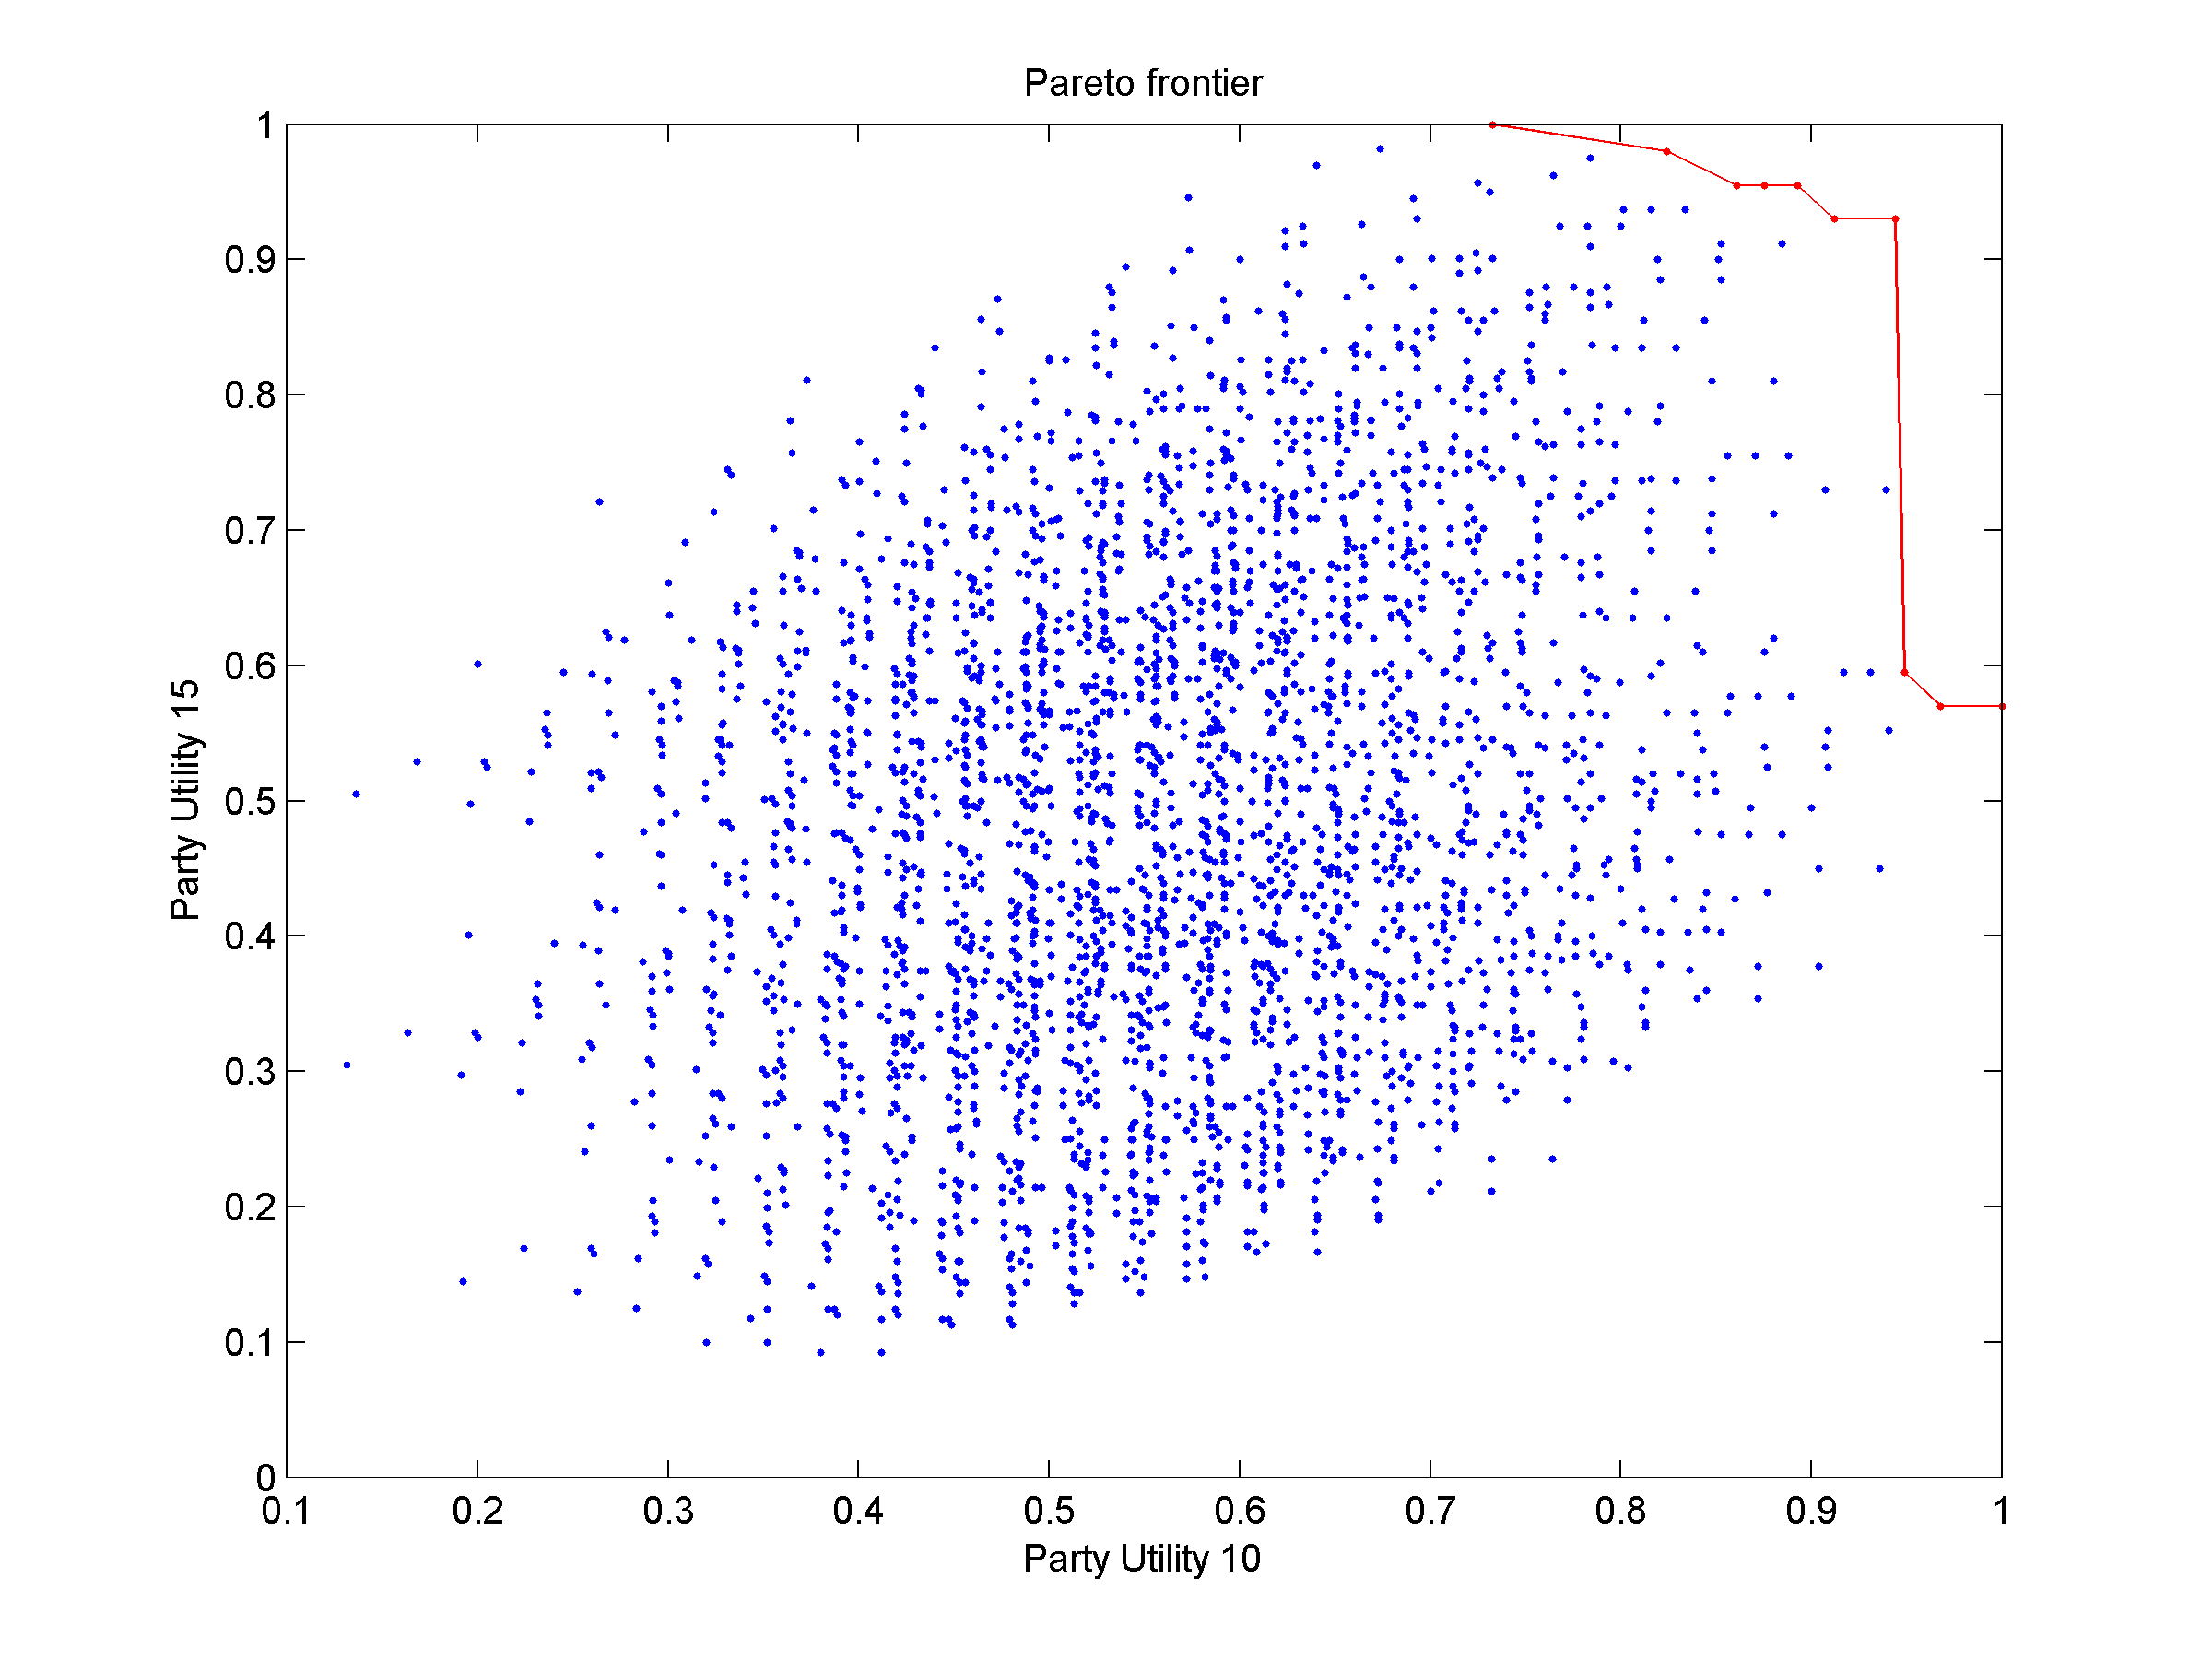
\includegraphics[width=0.8\textwidth]{pareto.png}
 \caption{The outcome space with the \emph{Pareto Optimal Frontier} indicated as a red line.}
 \label{fig:pareto} 
\end{center}
\end{figure}

\clearpage

\subsubsection{Performance of the \texttt{SimpleAgent}}

Finally, we perform two negotiation sessions: we play with the agent \texttt{SimpleAgent} against itself, and we play Boulware vs Conceder and discuss the outcome. When we play SimpleAgent against itself, we notice the behaviour is quite random. This is explained by having a loo at the code; it always offers a random bid higher than a certain threshold,
by default this threshold is zero. Therefore it performs a \emph{random walk} through the 
bidding space. The acceptance strategy works as follows: it calculates a probability for each bid and the higher the bid, the higher the probability. If the deadline approaches it will accept all bids with higher probability. It will however never accept bids with a utility of zero. The equation that determines the probability of acceptance is:
\begin{align}
P = \frac{u - 2ut + 2(-1 + t + \sqrt{((-1 + t)^2 + u(-1 + 2t)})}{-1 + 2t}
\end{align}

Where $P$ denotes the probability of acceptance, $u$ denotes the utility of the bid and $t$ denotes the time in a range of $[0, 1]$. Because of this behaviour we found the average utility playing against itself is around $0.68$, and the time needed to reach an agreement was very short: $0.03$ (averaged over $20$ negotiations on the party domain).
This is quite logical, since both sides offer random bids, it is the
case quite soon that either bid has a high probability of acceptance for the opposing party. When this agent negotiates with other agents, it performs badly, because
it offers random bids. Smart agents will accept good offers and deny other offers,
and because of this the obtained utility for the simple agent will be quite low.
We confirm this by letting simple agent play against Boulware. In these tests the simpleagent obtains an average utility of $0.6$ while the Boulware agent scores on average $1.0$. 

\subsubsection{Performance of the \texttt{Boulware} vs. \texttt{Conceder}}
Finally, we play with the Boulware agent against the conceder agent. A typical negotiation trace is displayed below: \\

\begin{figure}[H]
\begin{center}
 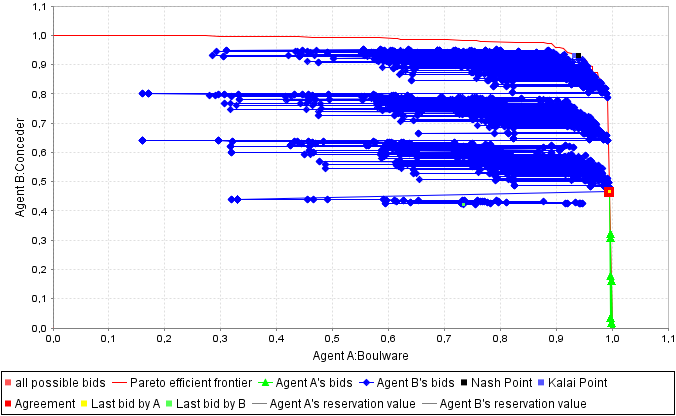
\includegraphics[width=0.9\textwidth]{traceConcederBoulware.png}
 \caption{The \emph{Pareto Optimal Frontier} is displayed with a red line in this figure.}
 \label{fig:pareto} 
\end{center}
\end{figure}

In this figure, the green and blue lines are the bidding-traces for respectively the Boulware and the Conceder agent. The boulware agent chooses the best bid for itself, and keeps offering this bid. This agent only concedes at the very last moments before the deadline. The conceder agent on the other hand starts conceding directly and keeps on conceding every new bid. We ran simulations on the party domain using these agents. Averaging over 20 negotiations the Conceder reached an utility of $0.67$ and
Boulware $0.99$. 
 
\subsection{PEAS Description}

The first step in designing an agent is to specify the environment as fully as possible. In order to do this we specify the PEAS description which lists the following aspects of the environment: \emph{Performance}, \emph{Environment}, \emph{Actuators} and \emph{Sensors}. This measure is extensively discussed in Russel and Norvig \cite{russel-norvig}, so we adapt their notation.

\begin{table}[H]
  \small
    \begin{tabular}{|p{1.8cm}|p{3cm}|p{3cm}|p{3cm}|p{3cm}|}
    \hline
    \textbf{Agent} & \textbf{Performance \mbox{Measure}} & \textbf{Environment} & \textbf{Actuators} & \textbf{Sensors} \\
    \hline
    BOA Agent & Own $($versus opponents$)$ discounted final utility & Negotiation space defined by Genius, \mbox{Opponents} & New bid offering, \mbox{accepting/rejecting} offers & Biddings of the \mbox{opponent} agent \\
    \hline
    \end{tabular}
    
    \caption{PEAS description for our negotiation agent \label{table:peas-description}}
\end{table}

Table~\ref{table:peas-description} displays the PEAS description for our agent. We will briefly discuss each of the descriptions. First the \emph{environment} our agent operates in, this is the negotiation space as defined by Genius. It contains all the possible bids, each resulting in an individual utility for the agents. The \emph{performance} is measured by the utility for the agent, which in this project has to be as high as possible $($with a maximum of $1)$ and preferably equal to or higher than the opponents utility. There are two \emph{actuators}, first of all the acceptance or rejection of a bid of an opponent. The second actuator is the offering of a new bid. The bid is based on the biddings of the opponent, which is the only \emph{sensor} the agent has. Under the surface of the PEAS elements, different java-classes, algorithms and calculations are performed, like the \textit{nash-point} and the \textit{Kalai-Smorodinsky solution}. These will be explained in more detail in the next sections.

\subsection{BOA Framework}

Most negotiation agents consist of three components: \emph{Bidding strategy}, \emph{Opponent model} and \emph{Acceptance strategy}. Together these three components form the \emph{BOA framework}. As discussed by Baarslag et al., the advantages of separating the components using this framework are threefold \cite{baarslag2012decoupling}. In designing our negotiation agent the most useful advantage was the fact that it allows for easily changing individual components and analyze the interaction between the components. Below we provide a small description for the three required components.

\begin{description}
  \item[Bidding Strategy] \hfill \\
  The bidding strategy is arguably the most important component. It's goal is to determine the next bid that will be offered to the opponent. In determining the next bid the agent can interact with the opponent model to provide a suitable offer. Sometimes the negotiation session is split up in multiple phases and each of the phases use a different bidding strategy.

  \item[Opponent Model] \hfill \\
  Analyzing the opponents behaviour is essential for being able to determine the opponent's preference profile.  With a well defined opponent model, the opponent's utility of a bid can be determined more accurate. In practice this works by estimating the opponents \emph{preference profile}, which is usually done by adapting \emph{Bayesian modeling} or \emph{frequency analysis}. 

  \item[Acceptance Strategy] \hfill \\
  Negotiation sessions ideally end by reaching an agreement. The acceptance strategy decides whether the opponents offer should be accepted or a new bid has to be offered. A broad variety of acceptance strategies is available with combinations of time-dependend, utility-dependent and threshold-dependent strategies.

\item[Opponent Model Strategy] \hfill \\
  Analyzing the opponents behaviour could, except for determining the opponent's preference profile, also be used to determine the strategy the opponent is using, like \emph{Hardheaded}, \emph{Conceder}, \emph{Tit-for-Tat}, etc. The own bidding strategy can be adapted to the opponent's strategy, to derive a maximum possible outcome for the own utility.

\end{description}

\section{Strategy}
\label{sec:strategy}

\subsection{Bidding Strategy}
\label{sec:strategyBS}
The bidding strategy we chose, is not a static strategy, but is time dependent. The strategy is divided in three different phases, with each phase using its own sub-strategy. The main \texttt{Group7\_BS} class decides the current phase by evaluating the normalized time (\texttt{getTime()}) and the two hard-coded phase thresholds, which are corrected for discounts and are stored in the array \texttt{phaseBoundary}. 
The phases itself are all subclasses of the \verb-Phase- class. In this section we discuss the strategy behind each of the phases separately. Note that, because we wanted our acceptance strategy and our opponent model (strategy) to 
work together, we have used a helper class (\verb-Helper-) as the BOA framework did not provide each component with references to all other components. Using the helper class, we can also share values, like the Kalai point, among all our components in order to save computation time and to allow other components to have access to otherwise unavailable information. In case our components are used separately, we ensure that we always have fall back values whenever we request a certain value from the helper class which could be unavailable, since the component that sets that value might be unavailable.

\subsubsection{First Phase}
By offering an opening bid of maximal utility, the opponent can easily estimate our preference profile. Due to this reason we have chosen to offer an initial bid of utility $1.0$ (lower values sometimes lead to bad results where this bid is extremely good for our opponent and is directly accepted).\\ 

After determining our opening bid and receiving the initial bid from the opponent, our agent continues by generating random bids. These random bids are generated within a small utility range (measured by our utility) given by the \verb-getBidRange-. The center of this range decreases by a small amount when time passes.
The center is first set to $1.0$, and ends at $0.9$ (the lower bound). The lowerbound is set to $0.9$, except when our opponent best bid is closer than $0.1$ to $0.9$ utility (in our utility scale). If this is the case the lower bound is set to the utility of this bid of the opponent $+0.1$, and we ensure that the lowerbound and upperbound do not overlap. The width of the range is set to  $0.02$. 

We do this, because we think that if the opponent can estimate our preference profile better,
we can reach better win-win situations. By conseding this way, we ensure that most opponent 
models accurately profile our preferences.

\subsubsection{Second Phase}

For phase $2$ we decided to implement the \emph{Tit-for-Tat} strategy \cite{titfortat}.
We chose this because it works fairly well against different agents, since you will play
hard against hardheaded opponents and more nice against conceding agents.
However, as noted in the referenced paper, we should not play too nice,
and try to exploit other opponents. We use the following strategy. \\

We use the distance to the \emph{Kalai-Smorodinsky} point as reference to calculate
the amount of concession for both the opponent as our own agent. When conceding, we aim for this point. We chose this point because we think it is the most fair since for this point
our utility is equal to the utility of the opponent.
We decided to use the distance to this point instead of only relying on our own utility 
or opponent estimated utilities, because when we look at these values we can hardly see whether or not our opponent is conceding: conceding opponents tend to vary a lot on the scale of our utility,
and utility estimates for the opponent are so noise one at least needs to average over more than 100 bids. So instead, we use the distance to the KS and this improves the detection of concessions,
since it relies on both the opponent model and our own utility estimates. \\

We average the change in distance (\verb-getAvgDifferenceKS-) of the last five bids to the Kalai-Smorodinsky point to determine the mean concession of the opponent. We
multiply this by a factor $\sfrac{1}{3}$, and then match their concession by walking towards the KS point. We multiply by this factor to avoid conceding too much in the direction of the opponent. 
We normalize every distance by taking the distance from the Kalai point to the best bid point of our agent and the opponent. We do a lineair interpolation between the best bid and the 
Kalai point (\verb-interpolateBidPoints-).
\\

Furthermore, to ensure our agent does not get stuck when playing against 
another Tit-for-Tat agent, we will randomly concede from time to time. 
These concessions are done towards the Kalai-Smorodinsky point, and linearly over 
$10$ bids, so the opponent can detect our concession more accurately. When the concession has been done, we hope the opponent matches  our concession. If the opponent has done this, we will approach him using Tit-for-Tat, but if not, we take our concession back. \\

Finally, we want to reach the most efficient outcomes. Because of this,
we will randomly offer bids on the \emph{Pareto Frontier} $50\%$ of the time (\verb-FindClosestParetoBidPoint()-).
However, to select this bid, we take the Pareto bid closest to our current bid in a special sense.
When determining the closest bid, we weigh our utility twice as much
as the opponent utility (\verb-interpolateBidPoints-), to ensure we don't concede too much by accident 
(this can happen when dealing with strange pareto frontiers).

\subsubsection{Third Phase}

The third phase only consists of the very last part of the negotiation session (usually from $t=0.95$). The strategy that is employed here offers bids that are decreasing when time elapses towards the end of the negotiation session, also the approximated opponent model strategy is used from our method \texttt{getOpponentModel()} in the OMS. \\

When this method returns that the opponent behaves as \emph{conceder} (\verb-ourHelper.getOMStrategy().getOpponentModel();-) then our agent chooses the best from two possibilities; the \emph{Kalai-Smodorinsky} point and the generated bid that decreases over time. When the opponent is assumed to be \emph{hardheaded}, then we just use the latter one. When this utility $u$ is determined we choose the best bid within the range $[u-0.01, u+0.01]$. Choosing the best bid is done by fetching all possible bids within this utility range and choosing the one that is best for the opponent by exploiting the information from our opponent model. This of course, increases the probability that the opponent accepts our bid. \\

Finding the best bid within the calculated utility range is not garantueed to succes, therefore we have also implemented a fallback mechanism. When determining the next bid has been tried for $15$ times, then a fallback bid is randomly chosen from already offered bids. This way we are sure that a bid is offered without wasting too much time.



\subsection{Opponent Model}
\label{sec:strategyOM}
Our opponent model is based on the standard \emph{frequency model}, but has some tweaks that attempt to improve the quality of the model. The issue weight estimation is still equal to the standard frequency model method. The difference is in the way we approximate values of the items within an issue. The improvement is based on the idea that if the opponent does a new, previously unseen, bid, that this is probably close in utility to the other bids we've seen. This is implemented by changing the so-called learn value addition based on how ``wrong'' our opponent model is for the current bid. \\

In order to estimate how ``wrong'' the estimate is, we first need to decide what offer we expect from the opponent. To do this we make the assumption that new offers the opponent makes are always close to old offers, but usually a bit lower. We also assume that the opponent's utility space has a normal distribution with a mean around $\mu = 0.5$, and a variance around $\sigma^2 = 0.02$. These values have been determined by examining some domains that were present in genius. The expected utility of a bid is calculated when we receive a bid we haven't received before from the opponent. We then look at how many distinct bids we have received ($D$) and what the size of the utility space is (the total number of bids possible, called $T$). We also approximate the average number of bids ignored by the opponent ($I$). We then use the quantile function of the normal distribution to calculate the expected utility:
\begin{align}
  E(U) = \text{normcdf}^{-1} \left(\frac{D \cdot I}{T}\right) = \mu + \sigma \sqrt{2} \cdot \text{erf}^{-1} \left(2 \frac{D \cdot I}{T} - 1\right)
\end{align}

Where $\text{erf}^{-1}(x)$ is the inverse \emph{error function}. We save this expected utility for each bid and use it again if the bid is made again. Next we check if the utility calculated using the current opponent model is within a certain range of the expected utility. If this is not the case we try a number of different learn value addition values ($1$ to $100$) and check for each of these values what the utility of the current bid would be if we used that value for the frequency modeling algorithm. We pick the learn value addition value that leads to the smallest absolute difference between the utility calculated using our opponent model and the expected utility. \\

The advantage of this method over standard value iteration is that it approximates the opponent model better for agents that are hardheaded. Bids that they have never done before leads to much bigger changes in the opponent model, which leads to a faster convergence towards to true opponent model. However, for agents that concede much faster then the algorithm anticipates (e.g. skip much more that $I$ bids whenever they make a new bid), the opponent model is less accurate. Since we found that most opponents are hardheaded for at least some part of the total time they are active, we think that, on average, this model will give better results.

\subsection{Acceptance Strategy}
\label{sec:strategyAS}
\todo{Ollibol, write something nice here... :-)}
% !TEX root = negotiation_final_report.tex
During the development of our acceptance strategy BOA component, $AC_{BOAconstructor}$, we designed, implemented, and tested many different acceptance conditions. Some failed horribly, but some exceeded our expectations. Within this paper we will only discuss the acceptance conditions that made it into the final product that was delivered along with this report.\\

Our acceptance strategy component consists of 7 acceptance conditions that are mainly based on the simple acceptance conditions as found in \cite{baarslag2013acceptance}. However, we modified these basic conditions according to our theories. To the best of our prior knowledge, they should all perform better together than any other acceptance strategy. Further along this report, we will discuss the tests we performed to evaluate our claims.\\

In the following subsections, we will discuss all 7 of our conditions included in our $AC_{BOAconstructor}$.

\begin{description}
  \item[AC Curve] \hfill \\
This acceptance condition is based on the simple $AC_{const}$\cite{baarslag2013acceptance}, but we added an extra dimension. $AC_{curve}$ depends on the normalized current time, $t_{current}$, of the negotiation and modifies the constant accordingly. We created a formula that would exponentially decrease when $t_{current}$ is close to $t_{end} = 1.0$ but would show almost non decreasing properties close to the beginning to the negotiation sessions. In the final version of $AC_{curve}$, we let it start at a utility boundary $f_{curve}(t = 0.0) = 1.0$, and approach the first bid of the opponent, $U_{other}^{1}$, so that $f_{curve}(t = 1.0) = (1 - \alpha) * 1.0 + \alpha * U_{other}^{1}$, where $\alpha$ is a percentage. This was preferred over approaching a static value, as it accommodates for varying preference profiles. However, we hereby assume that the opponent will most probably first send his best bid, in order to get his highest utility, namely $U_{opponent}^{1} = 1.0$. Until now we have not seen any agent that disagrees with this assumption, except the Simple Agent agent, which always selects a random bid. The value for $\alpha$ used in our final version is $\alpha = 0.5$.

  \item[AC Panic] \hfill \\
Our $AC_{panic}$ conditions is based on $AC_{time}$\cite{baarslag2013acceptance}, but instead of looking at a threshold for a normalized time value, we approximate the amount of bids that are possibly left and only accept after less than $\beta$ bids are left. This is done by calculating the time, $\Delta~t_{bid}$, that was needed for each bid, with the help of a running average. The remaining time, $t_{remaining} = 1 - t_{now}$, is divided by the averaged time per bid to get the amount of bids that are probably left: $\#_{bids left} = t_{remaining} / \Delta t_{bid}$. The value for $\beta$ used in our final version is $\beta = 3$.\\

Furthermore, 2 extra conditions were used before we accept with $AC_{panic}$. Firstly, if the last bid of the opponent was better than the perceived Kalai point minus a conceding value, say $\gamma = 0.05$, we accept for sure, since the received bid will be almost as good as a win-win or even better. Secondly, since we are in 'panic mode', we will also always accept when the opponent offers us a better offer than his best offer yet, minus the same conceding value $\gamma$.

  \item[AC Horror] \hfill \\
This condition is also based on $AC_{time}$, just like our previous condition. However, $AC_{horror}$ will always accept whenever we think that only 1 bid is left for us to propose, $\#_{bids left} = 1$, as it is always worse to end up with no agreement.

  \item[AC Kalai] \hfill \\
Whenever our utility of the opponent's last bid is really close to the Kalai point, $U_{kalai} - 0.01 <= U_{opponent}^{last} <= U_{kalai} + 0.01$, $AC_{kalai}$ always accepts, as this is a nice win-win situation. We only do this, though, when we are pretty sure that our calculated Kalai point is reliable. We do this by checking whether the opponent has made enough distinct bids to have an accurate enough opponent model.

  \item[AC Nash] \hfill \\
The acceptance condition $AC_{nash}$ is exactly the same as our $AC_{kalai}$, except for the use of the Nash point instead of the Kalai point.

  \item[AC Worst] \hfill \\
This condition is inspired on $AC_{next}$\cite{baarslag2013acceptance}, but instead of accepting when the received bid is higher than our next bid, we accept when the opponent's last bid is higher than our worst bid, minus an time-based increasing conceding value $\delta(t) = t * 0.05$, so that we accept when $U_{opponent}^{last} > U_{our}^{worst} - \delta(t_{now})$. However, to prevent this value from accepting too quickly, we created a time-dependent formula that we use to cut off the said threshold $U_{our}^{worst} - \delta(t_{now})$. The formula is defined as follows, $threshold(t) = max(\epsilon * (1-time) + \zeta, U_{our}^{worst} - \delta(t_{now}))$, where in our final version $\epsilon = 0.3$ and $\zeta = 0.6$. This way, our $AC_{worst}$ will never accept anything below a utility of 0.6, and when $t_{now} = 0.0$, the condition will never accept anything below 0.9.

  \item[AC Next] \hfill \\
The last acceptance condition is simply the $AC_{next}$ as mentioned in \cite{baarslag2013acceptance}.

\end{description}

Finally, our acceptance strategy only looks back within a sliding time window of $\omega = 0.2$, so that the behavior of most of the above mentioned acceptance conditions varies during the course of a negotiation session. This is to accommodate for changing behaviors in our and the opponent's strategies. Thus, we never look at the entire time line of a negotiation session, in order to determine the acceptability of the opponent's last bid.

\clearpage

\subsection{Opponent Model Strategy} 
\label{sec:strategyOMS}

While an opponent strategy model is not required for a good negotiation agent we have decided to implement a simple version of this component. Our strategy model has one method \texttt{getOpponentModel()} that approximates the behaviour of the opponent. \\

While testing our agent we noticed that \emph{hardheaded} opponents do not offer a large number of different bids, i.e. they stick to bids that have high utility for themselves. On the other hand, agents that act as \emph{conceder} offer a wide variety of bids due to their conceding behaviour. Our strategy model uses this information to determine the strategy of the opponent. \\

Our strategy model first fetches the bid history of the opponent, then these results are filtered on time. Only opponent bids that were offered before $t=0.6$ are taken into account. Then our helper function \texttt{getDistinctBids()} returns a list of unique bids, i.e. all different bids are returned only once. The number of distinct bids is compared to the total number of opponent bids by calculating the ratio between the two. This ratio is compared to a hardcoded threshold; empirical measurements suggested a threshold of $0.03$ for best results. A ratio below this threshold suggests the opponent to be \emph{hardheaded} since the number of unique bids is small. The method \texttt{getOpponentModel()} then returns that the opponent is hardheaded, while it returns \emph{conceder} otherwise. \\

For our agent, the classification (\emph{hardheaded} vs \emph{conceder}) of the opponent is sufficient. Initially our goal was to use this information in both the third phase of the bidding strategy and the acceptance strategy. However some tests indicated that using the opponent's strategy in the AS was not that useful. Therefore the strategy is only used in the last phase of the bidding strategy. \\

This is a very simple though efficient method for determining the opponents strategy. For future work we also suggest calculating the \emph{variance} between the opponents bids. A small variance would suggest the agent sticks to its own best utility and can be classified as hardheaded. This approach looks promising, however we did not have enough time to implement this.


\section{Testing \& Performance}
\label{sec:performance}
After designing and implementing our agent the BOAconstructor it is time to put it to the test in various situations. In the next two subsections we quantify the performance of our agent. We present the results of a wide range of tests and discuss the effeciency of the agent in terms of reaching \emph{Nash solutions} and outcomes that lie on the \emph{Pareto Optimal Frontier} (POF).

\subsection{Performance against \texttt{ANAC 2011} agents}

In this part we compare our agent to three of the agents that attended in the ANAC 2011 competitio: \emph{HardHeaded}, \emph{Gahboninho} and \emph{The Negotiatior}. In addition to those agents we also negotiate with ourself. The results have been obtained by running a tournament using multiple utility profiles for the Party domain and setting the negotiation time to $30$ seconds. \\

\begin{table}
	\centering
	\small
    \begin{tabular}{l|p{2cm}|p{2cm}|p{2cm}|p{2cm}|p{2cm}|p{2cm}|}
    ~              & Average Time Agreement & Average Discounted Util & Average Dist. to Nash & Average Dist. to Pareto & Average Dist. to Kalai \\
    \hline
    \emph{HardHeaded}		& 0.858  & 0.927  & 0.102  & 0.017  & 0.084   \\ \hline
    \emph{Gahboninho}   	& 0.887  & 0.918  & 0.032  & 0.001  & 0.035   \\ \hline
    \emph{The Negotiator} 	& 0.725  & 0.871  & 0.050  & 0.003  & 0.052   \\ \hline
    \emph{Self}             & 0.823  & 0.877  & 0.061  & 0.007  & 0.057   \\ \hline
    \end{tabular}
    \caption{Performance of our agent against \texttt{ANAC 2011} agents (Runtime: $30$s) \label{table:anac2011-results}}
\end{table}

From the results in Table~\ref{table:anac2011-results} we notice a fairly high average discounted utility against the other agents. Regarding the effiency of the negotiation we observe that the average distance to the \emph{Pareto Optimal Frontier} upon agreement is very small. When playing against \texttt{The Negotiator} we see than on average the agreement lies on the frontier.

\todo{Check these conclusions!}

\subsection{Choosing Different Acceptance Strategies}

The next test consists of running our agent with varying \emph{acceptance strategies}. We perform those test so we are able to compare our acceptance strategy with other available ones (our strategy is discussed in Section~\ref{sec:strategyAS}). Again these tests are performed by starting a small tournament. \\

\todo{Insert results and discuss them...}

\subsection{Comparison with HardHeaded Frequency Model}
To test if our opponent model is better than the default hardheaded frequency model, we ran the performance test against the ANAC 2011 agents using the hardheaded frequency model. The results of this are shown in \autoref{table:anac2011-hh}.
\begin{table}
	\centering
	\small
    \begin{tabular}{l|p{2cm}|p{2cm}|p{2cm}|p{2cm}|p{2cm}|p{2cm}|}
    ~              & Average Time Agreement & Average Discounted Util & Average Dist. to Nash & Average Dist. to Pareto & Average Dist. to Kalai \\
    \hline
    \emph{HardHeaded}		& 0.883  & 0.916  & 0.166  & 0.055  & 0.152   \\ \hline
    \emph{Gahboninho}   	& 0.881  & 0.848  & 0.116  & 0.020  & 0.097   \\ \hline
    \emph{The Negotiator} 	& 0.756  & 0.868  & 0.092  & 0.027  & 0.079   \\ \hline
    \emph{Self}             & 0.839  & 0.806  & 0.125  & 0.035  & 0.140   \\ \hline
    \end{tabular}
    \caption{Performance of our agent with \texttt{HardHeaded Frequency Modeling} (Runtime: $30$s) \label{table:anac2011-hh}}
\end{table}
We see that, compared to our own opponent model, the average utility has decreased by $0.071$, which means that our opponent model leads to  better results for our agents. 
Furthermore, we see that the average utilities for the opponent are also lower compared to what our opponent model achieved.
The distance to the Nash point, Pareto frontier and Kalai point are especially interesting for evaluating the quality of the opponent model: a better opponent model allows us to do bids closer to these optimal values. We also note here that for every agent these properties are lowest using our own opponent model.

\subsection{Performance In Different Domains}
In order to test whether our agent can cope with different domains, we tested it against the same selection of 2011 agents, but using different domains. More specifically, the test was run in the Car/ADG domain, the Amsterdam party domain, the Camera domain, the Nice Or Die domain, the Grocery domain, the IS BT Acquisition IS prof domain, and the Laptop domain. The average results for all agents are shown in \autoref{table:anac2011-domains}.
\begin{table}
  \centering
  \small
  \begin{tabular}{l|p{2cm}|p{2cm}|p{2cm}|p{2cm}|p{2cm}|}
    ~ & Average Time Agreement & Average Discounted Util & Average Dist. to Nash & Average Dist. to Pareto & Average Dist. to Kalai \\
    \hline
    HardHeaded & 0.807 & 0.750 & 0.142 & 0.032 & 0.150 \\
  Gahboninho & 0.731 & 0.807 & 0.065 & 0.004 & 0.165 \\
  The Negotiator & 0.694 & 0.646 & 0.288 & 0.000 & 0.220 \\
  Self & 0.744 & 0.712 & 0.165 & 0.012 & 0.179 
  \end{tabular}

\end{table}



\subsection{How Generic is our Agent?}

In the previous tests we only observed the behaviour of the agent on the party domain. In order to test how generic our agent is we also perform a number of tests on other scenarios. In addition to different domains we also incorporate \emph{discounts} for the utility. \\
\todo{Insert test results and discuss results...}





\section{Conclusion}
\label{sec:conclusion}


For this project we performed an in-depth study in the world of automated negotiation. After reading a large amount of literature written about the subject we have designed and implemented our own agent using the BOA framework and \texttt{Genius} environment. It became clear to us that negotiation is not as straight forward as it might seem at first glance. Reaching an agreement that is a win-win situation for both parties can be quite hard.

Our agent, the BOAconstructor, combines multiple existing ideas.
However, we tried to implement the tit-for-tat strategy which was very hard to get to work properly, and we have also introduced multiple phases that introduced a lot of parameters. Our resulting agent is very complex, and because of this we had many difficulties optimizing the parameters of each of our components because of the high dimensional parameter search space.
Also because of the complexity there were a lot of bugs, which limited our testing time considerably. Because of this, our agent is clearly performing suboptimal. In the tests we have seen that our acceptance strategy in combination with the third phase of our bidding strategy almost always leads to acceptance, which is apparently a tad too lenient when facing most other agents. Furthermore, we found that many settings we tried for phase two, led to a rapid concession compared to our opponent.  Therefore, we have decided to disable these concessions in final tests. Sadly, we did not have time to optimize these parameters further.

We conclude that in automated negotiation, starting out with a simple agent and 
continually improving this agent, would have been a better strategy to develop agents. 
We clearly started out with a too complex agent before optimizing any parameters.
However, we think that separating a bidding strategy into phases can lead to 
better results than just using a single bidding strategy. By adding parameters
to each individual phase, we can explore the space of strategies even more
than just using a BOA agent.

Our mistakes might be in part because of the too large separation between members of our project group.
Each of us often worked on our 'own' component, and because of this, most of us made components too complex as there was no overview. Furthermore, we had some practical issues with version control, from which we learned a lot.
Finally, we have really enjoyed this challenge, although we aren't entirely satisfied with 
our results. We wish we could spend more time on this project looking back at our mistakes,
since we think our agent can be improved a lot.
 
\section{Future Perspectives}
\subsection{Improving BOA constructor}
During the development of the BOAconstructor agent, we found that there are features that could improve the results, but we didn't have time to implement. This happened for each of the BOA components.

The Bidding Strategy phase 2 has too many parameters which are not correctly optimized.
The agent could be considerable improved by this optimization. Furthermore, 
the last phase is also not fully optimized, sometimes conceding too much.

The Opponent Model now still uses default frequency modeling for adjusting the issue weights. Estimating the issue weights using a system similar to the one used to estimate the value weights might lead to improved results. Another method to potentially improve the results is to cross check whether the learn rate used doesn't brake the estimates for previous offers. In other words: check if after the value iteration the estimates of all previous bids are still within range of the expected utility. 

Our Acceptance Strategy uses many acceptance conditions which in some cases overlap. We can imagine that we could leave out one or two of these conditions. However, our results are promising, as we seem to get the highest utility when we use our own acceptance strategy. This is not surprising though, since we take a lot of cases into account. This makes our acceptance strategy really complex, and by optimizing the parameters and refactoring the code we could possibly reduce its complexity. We suggest to test each condition and its parameters separately, in order to find out if they actually improve or worsen our results.

\subsection{Future of BOA constructor for real-life negotations}
Before our agent -- or most negotiation agents -- can be used by humans in real negotation 
session, we think a lot has to be done. People probably want more control over the 
negotiation process of the agent, and specifically in understandable terms, e.g. no hard but fuzzy parameters.
Also it is important for people to understand what it is doing. 
Tutorials to see that the agent is performing well would be important. 
This might be best realized by letting people negotiate against the agent. 
This could illustrate the different tactics of the agent and give an idea of it's settings.

\subsection{Using a mediator}
In the process of optimizing the agent to reach the best possible outcome of the negotiation session, it turned out to be hard to find a deal that is Pareto optimal. Another way of negotiating is by using a mediator, which objectively mediates between two or more agents. The agents which take part of the negotiation all get the same bid from the mediator, which the agents can accept or reject. This means that the \textit{bidding} actuator is now canceled, the only actuator now is \textit{accepting/rejecting}.

Since agents can only reject or accept a bid of the mediator, so seeing no bids of the opponents, it is very hard to make a preference profile of the opponents. Therefore, it is most probable that agents will focus on their own utility. Besides that, agents won't care much about the utility of the other agent as long as they get a good utility themselves. 

Since the mediator has both preference profiles, it is able to calculate all the bids on the Pareto frontier including the \emph{Nash-point} and the \emph{Kalai-Smorodinsky solution}. An objective mediator can walk over the Pareto Optimal Frontier, offerings bids until both agents accept. An objective negotiation should end in the Nash-point or Kalai-Smorodinsky point. However, since we are at the optimal frontier, the first bid which is accepted by both parties will be the outcome.

This way of negotiating will compute an optimal outcome, however in a restricted optimal outcome space. There are less possibilities for strong negotiating agents to influence and analyze the opponent, so they could get a worse outcome. Especially in bidding spaces which are poorly distributed in favor of one agent, the agent will probably get a worse outcome.

So in conclusion, we think that it can be useful if both parties want to reach an optimal outcome.
However, if one of the negotiators wants to exploit the opponent, or just negotiate, a mediator
is not the solution, because it hardly allows for any real negotiation.

\subsection{Other possibilities to improve automated agents}
Extending agents with more communication abilities would probably not increase the performance significantly. They could
communicate about certain issues, for example if they would concede or stay. However, it will never be sure when an agent is telling the truth or using a communication strategy. 

Communication that however could be useful, is communication about what agents do not want. After communicating this, agents could neglect certain offers to shrink the negotiation space. This could save time, and could be useful when there is a time constraint or a discount factor. 

However, another way to look at this is that the domain could be specified better at the start of the negotiation, by filtering the issues which never would be accepted by the opponent beforehand. For example, when buying a car, one could have a default domain where all possible values for all possible cars are specified, which is 
downloaded to your pocket negotiator. Then it would be useful to remove all the cars without certain features, so which are not matching your preferences, beforehand. 

There are also other possibilities. Considering humans when negotiating, they are able to offer issues outside the negotiation domain, to convince the opponent to get this deal. Well known examples are money or, in the case of cars, extra tires. In the current \texttt{Genius} environment it is impossible to offer new issues in a negotiation session, maybe this could be a feature in the future when negotiators are able to rate unknown issues or when they can ask for input of a human. 

\subsection{Feedback concerning genius}

Because our agent's quite complex behavior, we tried to use as much functions
already in the Genius API to reduce our workload. However, using the Genius API 
sometimes was very challenging. Below we make a short list of issues we encountered,
which -- we hope -- can be used to improved the next versions of Genius:

\begin{itemize}
\item It was not possible for our acceptance strategy to communicate with the 
opponent model strategy or opponent model. This is a real problem, 
since for acceptance we wanted to check if bids were pareto optimal and so forth
before accepting. Therefore, we created our \texttt{Helper} class.
\item Conversions between \verb-bidDetails-, \verb-bid- and \verb-bidPoint- classes can be hard. Especially 
converting \verb-bidPoints- back to bid or \verb-bidDetails- seemed impossible, we had to search through
part of the bid-space to find back the bids corresponding to \verb-bidPoints-, as the \texttt{BidPoint.getBid()} method returned \texttt{null}.
\item Built in functions of the opponent's \verb-utilitySpace- do not work for all default included 
opponent models. For example, the Bayesian model does not construct a \verb-utilitySpace- for the opponent. 
In fact, we were not able to construct utility spaces for most models except the hardheaded frequency model. 
\item \verb-Bid-s do not calculate a hash code that gives the same results as the equals function. This would 
be useful for creating a \verb-Dictionary-/\verb-HashMap- where bids are mapped to utilities.
\item It is very hard to retrieve the value names within the issues from the domain (if not impossible).
\item The function to calculate the Kalai-Smorodinsky point, which we used intensively,
does not always return the correct bid. This is best demonstrated in the domain 
\verb-NiceOrDie-, where it returns the ``Die'' offers as being the Kalai-Smorodinsky point if the opponent model
is not entirely correct, but slightly skewed.
\item In Genius, when running tournament a second time, log files are not correctly saved.
It will try to append the new log file to the old one, and because of this genius will throw
an exception. 
\item In Genius, when loading tournaments or adding agents, the parameters are suddenly scrambled and don't comply to their original order. Also the descriptions are not saved or loaded, so one can not easily interpret the meaning of the parameters anymore. the only fix is to reselect the component, in order to load the descriptions and get the original order back.
\item In Genius, when editing parameters of BOA components, the labels for the parameter names are super small and only display the first few characters. This is especially frustrating with the issue mentioned above.
\item It would be very nice if one could export a whole trace of values from a negotiation
session for analysis and debugging. We have implemented a logging BOA component to do this for us, but this worked very inefficient.
\item When executing a tournament, it would be nice if it was shown in the results table what agent accepted a bid.
\item Columns \texttt{AgentA params} and \texttt{AgentB params} are always empty and all parameters are summarized in the agent names instead, making the former 2 columns obsolete.
\end{itemize}



\bibliography{negotiation_final_report}
\bibliographystyle{plain}

\end{document}
